In this chapter, we make a compromise and provide an introduction to the field of digital circuits that introduces only the necessary concepts to understand the principles on which the organization and architecture of computers are based. We generally present functional or behavioral designs in preference to highly optimized structural components.

%%%%%%%%%%%%%%%%%%%%%%%%%%%
\section{Boolean Algebra}
%%%%%%%%%%%%%%%%%%%%%%%%%%
Boolean algebra is a branch of mathematics that deals with binary variables and logical operations. It serves as the foundation for modern digital logic and computer science, enabling the design and analysis of digital circuits and computational algorithms. Developed in the mid-19th century, Boolean algebra forms the basis of everything from simple electronic gates to complex processors.

%*********************************
\subsection{Historical Background}
%*********************************
Boolean algebra was introduced by George Boole in \emph{An Investigation of the Laws of Thought}, published in 1854 \cite{boole1854book}. Boole sought to formalize the process of human reasoning using a symbolic language, representing logical relationships through algebraic structures. Although initially developed as a tool for philosophy and logic, Boolean algebra found practical applications in the early 20th century when Claude Shannon demonstrated its utility in designing electrical circuits \cite{shannon38}.

Shannon's master's thesis, \emph{A Symbolic Analysis of Relay and Switching Circuits}, linked Boolean algebra with electrical switches, showing how logical operations could be implemented using relay circuits. This work laid the foundation for digital circuit design and the development of modern computers \cite{shannon38}.

%***********************
\subsection{Basic Concepts}
%************************
Boolean algebra operates on a binary set \( B = \{0, 1\} \), where:
\begin{itemize}
    \item \( 0 \) represents \textbf{false}.
    \item \( 1 \) represents \textbf{true}.
\end{itemize}

%*******************
\subsection{Operations}
%*******************
\paragraph{AND (\( \land \)).} A binary operation where \( A \land B = 1 \) if and only if both \( A = 1 \) and \( B = 1 \).
\paragraph{ OR (\( \lor \)).}  A binary operation where \( A \lor B = 1 \) if at least one of \( A \) or \( B \) equals \( 1 \).

\paragraph{NOT (\( \neg \)).} A unary operation where \( \neg A = 1 \) if \( A = 0 \), and \( \neg A = 0 \) if \( A = 1 \).

%*****************
\subsection{Laws}
%*****************
These operations obey the following basic laws:
\paragraph{Commutative Law:} 
\[
A \lor B = B \lor A, \quad A \land B = B \land A
\]

\paragraph{Associative Law:} 
\[
A \lor (B \lor C) = (A \lor B) \lor C, \quad A \land (B \land C) = (A \land B) \land C
\]

\paragraph{Distributive Law:} 
\[
A \land (B \lor C) = (A \land B) \lor (A \land C)
\]

\paragraph{Identity Law:} 
\[
A \lor 0 = A, \quad A \land 1 = A
\]

\paragraph{Complement Law:} 
\[
A \lor \neg A = 1, \quad A \land \neg A = 0
\]

%***************************
\subsection{DeMorgan's Laws}
%***************************
Augustus De Morgan (1806–1871) was a British mathematician and logician whose work played an important role in the development of formal logic and algebra. Born in India and educated in England, De Morgan became the first professor of mathematics at University College London \cite{grattan1997}. 

De Morgan's Laws were introduced in his 1847 book, \emph{Formal Logic: or, The Calculus of Inference, Necessary and Probable} \cite{deMorgan1847}. In this work, De Morgan formalized rules for distributing negations over logical operators, providing a foundation for algebraic reasoning in logic. While the concepts underlying these laws can be traced back to Aristotelian logic, De Morgan was the first to formalize them using algebraic symbols.

His work paralleled that of George Boole, whose algebraic system, now known as Boolean algebra, was published in the same period. Together, De Morgan and Boole changed the field of logic, moving it from a purely philosophical discipline to a mathematical one \cite{grattan1997}.

DeMorgan's Laws are fundamental principles in Boolean algebra, describing the relationships between logical conjunction (AND), disjunction (OR), and negation (NOT). They provide a way to express the complement of a compound expression in terms of the complements of its components. These laws are especially useful in digital logic design and simplification, as they allow for the transformation of logic expressions to equivalent forms using fewer gates or alternate gate configurations \cite{rosen2018, tanenbaum2013}.

Mathematically, DeMorgan's Laws state:
\[
\neg (A \lor B) = (\neg A) \land (\neg B), \quad \neg (A \land B) = (\neg A) \lor (\neg B)
\]

These laws can be proven using truth tables or algebraic manipulation and hold for any Boolean variables \( A \) and \( B \). In words:
\begin{itemize}
    \item The complement of a disjunction (\( A \lor B \)) is equivalent to the conjunction of the complements (\( \neg A \land \neg B \)).
    \item The complement of a conjunction (\( A \land B \)) is equivalent to the disjunction of the complements (\( \neg A \lor \neg B \)).
\end{itemize}

%**********************************************
\subsubsection{Applications of DeMorgan's Laws}
%**********************************************
DeMorgan’s Laws are widely applied in the simplification and design of digital circuits. For example, consider the simplification of the following expression that enables the implementation of the logic using AND gates and inverters rather than a more complex combination of gates \cite{rosen2018, karnaugh1953}.
\[
\neg (A \lor B \lor C) = \neg A \land \neg B \land \neg C
\]

%******************************************
\subsection{Applications in Digital Logic}
%*****************************************
Boolean algebra provides the mathematical framework for designing and analyzing digital circuits. Logical gates such as AND, OR, and NOT are implemented in hardware to perform the basic operations of Boolean algebra. More complex circuits, such as multiplexers, decoders, and arithmetic logic units (ALUs), are built using combinations of these gates.

%*************************************************
\subsubsection{Simplification of Logic Expressions}
%*************************************************
One of the uses of Boolean algebra in digital logic is the simplification of logic expressions to minimize the number of gates required in a circuit. Simplification methods include:

\begin{itemize}
    \item \textbf{Boolean identities}: Using the laws of Boolean algebra to rewrite expressions  to convert between AND-OR logic and NAND-NOR logic \cite{rosen2018}.
    \item \textbf{Karnaugh maps}: A graphical method for simplifying logic functions \cite{karnaugh1953}.
    \item \textbf{Quine-McCluskey algorithm}: A tabular approach to minimize logic expressions \cite{quine1952}.
\end{itemize}

%%%%%%%%%%%%%%%%%%%%%%%
\section{Truth Tables}
%%%%%%%%%%%%%%%%%%%%%%%
Truth tables are a fundamental tool in Boolean algebra, logic, and digital circuit design. They provide a systematic way to represent and analyze the behavior of logical expressions and digital circuits by listing all possible input combinations and their corresponding output values \cite{rosen2018, tanenbaum2013}.

%****************************************************
\subsection{Definition and Structure of Truth Tables}
%****************************************************
A truth table is a tabular representation of a logical expression or circuit. It includes the following components:
\begin{itemize}
    \item Input Variables: Columns representing the logical variables (\( A, B, \ldots, N \)).
    \item Output Values: Columns representing the result of applying a logical operation or expression to the input variables.
    \item Rows: Each row corresponds to a unique combination of input variable values, covering all \( 2^n \) possible combinations for \( n \) variables.
\end{itemize}

For example, the truth table for a simple AND operation (\( A \land B \)) is as follows:
\[
\begin{array}{|c|c|c|}
\hline
A & B & A \land B \\
\hline
0 & 0 & 0 \\
0 & 1 & 0 \\
1 & 0 & 0 \\
1 & 1 & 1 \\
\hline
\end{array}
\]

%****************************************************
\subsection{Logical Operators and Their Truth Tables}
%****************************************************
Truth tables are used to describe the behavior of basic logical operators. The primary logical operations include:
\begin{itemize}[noitemsep, topsep=0pt]
    \item NOT (\( \neg \)): Negation inverts the value of a single variable.
    \[
    \begin{array}{|c|c|}
    \hline
    A & \neg A \\
    \hline
    0 & 1 \\
    1 & 0 \\
    \hline
    \end{array}
    \]
    
    \item AND (\( \land \)): Returns true if both inputs are true.
    \[
    \begin{array}{|c|c|c|}
    \hline
    A & B & A \land B \\
    \hline
    0 & 0 & 0 \\
    0 & 1 & 0 \\
    1 & 0 & 0 \\
    1 & 1 & 1 \\
    \hline
    \end{array}
    \]
    
    \item OR (\( \lor \)): Returns true if at least one input is true.
    \[
    \begin{array}{|c|c|c|}
    \hline
    A & B & A \lor B \\
    \hline
    0 & 0 & 0 \\
    0 & 1 & 1 \\
    1 & 0 & 1 \\
    1 & 1 & 1 \\
    \hline
    \end{array}
    \]

    \item XOR (\( \oplus \)): Returns true if exactly one input is true.
    \[
    \begin{array}{|c|c|c|}
    \hline
    A & B & A \oplus B \\
    \hline
    0 & 0 & 0 \\
    0 & 1 & 1 \\
    1 & 0 & 1 \\
    1 & 1 & 0 \\
    \hline
    \end{array}
    \]
\end{itemize}

%****************************************
\subsection{Applications of Truth Tables}
%****************************************
Truth tables are used in various domains of computer science, mathematics, and engineering:
\begin{enumerate}
    \item Expression Simplification: Truth tables help simplify logical expressions by identifying equivalent forms.
    \item Circuit Design: In digital electronics, truth tables describe the behavior of combinational circuits such as multiplexers, decoders, and adders.
    \item Validation and Verification: Logical correctness of algorithms and circuits can be validated using truth tables.
    \item Set Theory and Predicate Logic: Truth tables are used to analyze logical relationships and implications in formal proofs.
\end{enumerate}

%*************************************************************
\subsection{Constructing Truth Tables for Complex Expressions}
%*************************************************************
For complex expressions involving multiple variables and operators, truth tables are constructed by evaluating the expression step-by-step:
\begin{enumerate}
    \item List all possible input combinations (\( 2^n \) rows for \( n \) variables).
    \item Break the expression into subexpressions and calculate their values row by row.
    \item Combine subexpression results to compute the final output.
\end{enumerate}

For example, consider \( \neg (A \lor B) \land C \). The truth table is as follows:
\[
\begin{array}{|c|c|c|c|c|c|}
\hline
A & B & C & A \lor B & \neg (A \lor B) & \neg (A \lor B) \land C \\
\hline
0 & 0 & 0 & 0 & 1 & 0 \\
0 & 0 & 1 & 0 & 1 & 1 \\
0 & 1 & 0 & 1 & 0 & 0 \\
0 & 1 & 1 & 1 & 0 & 0 \\
1 & 0 & 0 & 1 & 0 & 0 \\
1 & 0 & 1 & 1 & 0 & 0 \\
1 & 1 & 0 & 1 & 0 & 0 \\
1 & 1 & 1 & 1 & 0 & 0 \\
\hline
\end{array}
\]

%****************************************
\subsection{Limitations of Truth Tables}
%****************************************
While truth tables are highly effective for small-scale problems, their size grows exponentially with the number of variables (\( 2^n \) rows for \( n \) variables). This makes them impractical for analyzing complex systems with a large number of inputs. In such cases, alternative methods such as Karnaugh maps, Quine-McCluskey algorithms, or software tools are employed \cite{karnaugh1953, rosen2018}.


%%%%%%%%%%%%%%%%%%%%%%%%%%%%%%%%
\section{Digital Domain}
%%%%%%%%%%%%%%%%%%%%%%%%%%%%%%%%
%******************************************
\subsection{Signals in the Digital Domain}
%******************************************
In the electronic digital domain, we work with only two values (see Figure \ref{fig:logic_levels}):

\placedrawing[H]{figures/01_01_digital_0_and_1.lp}{The two levels of the signal in the digital domain. Low level (0 Volt) for {\tt 0} or {\tt false}, and high level ($V_{DD}$ Volt) for {\tt 1} or {\tt true}.}{fig:logic_levels}

\begin{itemize}
\item 0, represented by the electrical value 0 V, having two meanings:
\begin{itemize}
\item the numerical value {\tt 0}
\item the logic value {\tt false}
\end{itemize}
\item 1, represented by the electrical value $V_{DD}$ V, having two meanings:
\begin{itemize}
\item the numerical value {\tt 1}
\item the logic value {\tt true}
\end{itemize}
\end{itemize}

The signals used in a digital system are of two types:
\begin{itemize}
\item non-periodic, with a certain structure ("random") adapted to the process of simulating the operation of a digital system
\item periods, usually with a strictly alternating structure, used as clock signals by which the operation of a digital system is synchronized.
\end{itemize}

Any simulation is based on the generation of waveforms with which the simulated circuit is stimulated on its inputs. We describe two generated waveforms: one "random" and one usable as a periodic signal.

%###################
% WaveformGenerator
%###################
\ifthenelse{\boolean{chiselversion}}{
%*************************************************
\subsubsection{Chisel Implementation of Waveforms}
%*************************************************
\includechiselcode[caption={Waveform Generator Code (Chisel)},     label={lst:chisel_waveformgenerator}, firstline=8, firstnumber=8, lastline=24]{\chiselSourceDir/waveFormGenerator.scala}

Listing \ref{lst:chisel_waveformgenerator} shows a Chisel version of a \texttt{WaveFormGenerator} module with two distinct output waveforms: \texttt{randomWave} and \texttt{clockWave}. Both signals are driven by internal logic that determines their behavior over time.

The \texttt{randomWave} signal is defined as a repeating sequence of Boolean values: \texttt{false}, \texttt{true}, \texttt{false}, \texttt{true}, and \texttt{false}. A register, \texttt{randomIndex}, is used to track the current position in this sequence. The module cycles through the sequence in order, and when the last value is reached, the index resets to zero, causing the pattern to loop indefinitely. 

The \texttt{clockWave} signal generates a toggling clock with a period of two cycles. This is achieved using a register, \texttt{clockToggle}, which alternates between \texttt{true} and \texttt{false} on each clock cycle. The result is a square wave output that can be used as a clock signal for other hardware modules or for synchronization purposes.

The \texttt{WaveFormGenerator} module demonstrates the generation of simple waveforms using high-level constructs in Chisel. By abstracting away low-level timing details, it provides a clean and maintainable implementation suitable for hardware design and simulation.

\begin{figure}[H]
    \centering
    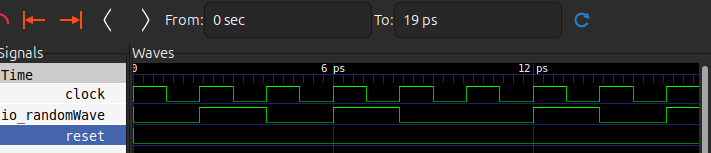
\includegraphics[width=\textwidth]{Images/verilator_waveformgenerator_screenshot.png} 
    \caption{Waveforms for generated SystemVerilog Verilator simulation}
    \label{fig:verilator_wave}
\end{figure}

\includechiselcode[caption={Waveform Generator Code with Emit SystemVerilog (Chisel)},     label={lst:chisel_waveformgenerator_emit_sv}, firstline=26, firstnumber=26, lastline=29]{\chiselSourceDir/waveFormGenerator.scala}

Chisel has the capability to emit SystemVerilog, Verilog, Waveforms (vcd), and circuit diagrams (svg). Section \ref{sub:verilator_test_driver} shows the process for generating the waveform shown in Figure \ref{fig:verilator_wave}. It uses Verilator rather than internal Chisel output.
}%end chisel

\ifthenelse{\boolean{verilogversion}}{
%*********************************************************
\subsubsection{SystemVerilog Implementation of Waveforms}
%*********************************************************    
\includeverilogcode[caption={Waveform Generator Code (Hand Written Verilog)},     label={lst:verilog_waveformgenerator}, firstline=8, firstnumber=8, lastline=999]{\verilogSourceDir/waveFormGenerator.sv}

Listing \ref{lst:verilog_waveformgenerator} shows the hand written SystemVerilog module, \texttt{waveFormGenerator}. It generates two output waveforms: a \texttt{randomWave} signal and a \texttt{clock} signal. The \texttt{randomWave} signal transitions between predefined states based on explicit delays specified using the \texttt{\#} operator. It begins at \texttt{0}, transitions to \texttt{1} after 2 time units, back to \texttt{0} after 6 more time units, to \texttt{1} after 4 additional time units, and finally to \texttt{0} after 8 time units. The simulation halts 5 time units later using the \texttt{\$stop} command. The \texttt{clock} signal is a periodic waveform toggling its state every 2 time units, implemented with a \texttt{forever} loop.

\placedrawing[H]{figures/01_02_waveSim.lp}{Waveforms generated by Vivado for hand written SystemVerilog simulation}{fig:vivado_wave}

Figure \ref{fig:vivado_wave} shows the results of simulating the {\tt waveFormGenerator.sv} module using Vivado.

}%end verilog

\ifthenelse{\boolean{verilogversion} \and \boolean{chiselversion}}{   
%*********************************************************************************
\subsubsection{Comparison of Chisel and SystemVerilog Implementation of Waveforms}
%**********************************************************************************
In the Chisel implementation of the \texttt{waveFormGenerator}, the functionality is expressed using high-level abstractions. The \texttt{randomWave} is generated as a cyclic sequence of Boolean values, and its transitions are determined by a counter that increments on every clock cycle. Unlike the Verilog version, the Chisel implementation does not explicitly emulate timing delays but instead assumes uniform timing for each state in the sequence. 

While both implementations generate a \texttt{randomWave} and a clock-like signal, they differ in their timing behavior and functionality. The Verilog version explicitly specifies time delays for signal transitions and provides a clear stop condition using \texttt{\$stop}. The Chisel version is higher-level, more abstract, and assumes regular timing intervals without emulating the exact delays. This makes the Chisel version more suitable for hardware synthesis, where timing is managed by the clock, while the Verilog version offers precise control for simulation purposes.
}%end both true

%%%%%%%%%%%%%%%%%%%%%%%%%%%%%%%%%%%%%%%%%%%
\section{One-Input Combinational Circuits}
%%%%%%%%%%%%%%%%%%%%%%%%%%%%%%%%%%%%%%%%%%%
Combinational circuits are a fundamental type of digital circuit where the outputs are determined solely by the current inputs, without any memory or feedback elements. They perform logical and arithmetic operations based on Boolean algebra. Examples of combinational circuits include logic gates (AND, OR, NOT), arithmetic circuits (adders, subtractors), and data routing components (multiplexers, encoders). These circuits are deterministic, meaning their outputs are uniquely determined by the given inputs \cite{mano2017}.

%******************************
\subsection{Formal Description}
%******************************
A one-input combinational circuit is a digital logic circuit where the output depends solely on the value of a single binary input \( A \). Such circuits are governed by a Boolean function \( f(A) \), where \( f: \{0, 1\} \to \{0, 1\} \). The output is computed instantaneously based on the input value, with no memory or feedback elements involved. The behavior of the circuit can be described by a truth table, which enumerates the two possible input values (\( A = 0 \) and \( A = 1 \)) and their corresponding outputs (\( f(0) \) and \( f(1) \)). 

\begin{table}[H]
  \begin{center}
    \caption{One-input circuits.}
    \label{tab:one_input_circuits}
    \begin{tabular}{|c||c|c|c|}
      \hline
      A&  &  NOT&  BUFFER      \\ \hline \hline
      0&  &   1&       0    \\ \hline
      1&  &   0&       1    \\ \hline
    \end{tabular}
  \end{center}
\end{table}

\placedrawing[H]{figures/02_01_not.lp}{Graphic representation of the NOT and BUFFER circuits.}{fig:one_input_ckt}

Table \ref{tab:one_input_circuits} shows the truth table for a NOT gate, which inverts the input (\( f(A) = \neg A \)), and BUFFER (constant) circuit, which outputs a fixed value regardless of the input (\( f(A) = 0 \) or \( f(A) = 1 \)). Figure \ref{fig:one_input_ckt} shows the logic circuit symbol of the NOT and BUFFER combinational circuits. This is also called a gate symbol.

%***************************************************
\subsection{Physical Implementation of NOT Circuit}
%***************************************************
The physical implementation of a NOT circuit, or inverter, bridges the abstract concept of Boolean algebra with real-world digital hardware. A NOT gate takes a single input and produces an output that is its logical complement. In practice, this is typically achieved using transistor-based designs, such as CMOS (Complementary Metal-Oxide-Semiconductor) technology. 

The delay inherent in a NOT circuit, commonly referred to as the \emph{gate delay}, arises from the physical properties of the transistors and the interconnects. When the input changes state, the transistors must charge or discharge the capacitive load at the output. This charging and discharging process is influenced by factors such as the capacitance of the output node, the resistance of the transistors, and the speed of the power supply. As a result, the propagation delay, defined as the time taken for the output to reach a certain percentage of its final value after a change in input, becomes an important metric in digital circuit performance. 

Understanding where gate delays originate is important for designing circuits that meet timing requirements in high-speed applications. The interested reader can consult Appendix \ref{app:physical_implementations} for more information.

%%%%%%%%%%%%%%%%%%%%%%%%%%%
\section{Two-input gates}
%%%%%%%%%%%%%%%%%%%%%%%%%%%
Two-input gates depend on two binary inputs. Common two-input gates include AND, OR, XOR, NAND, and NOR. 

%*******************************
\subsection{Formal Description}
%******************************
Two-input gates are fundamental components in digital logic that perform Boolean operations on two binary variables, \( A \) and \( B \), to produce a single output \( f(A, B) \). Mathematically, these gates implement functions \( f: \{0, 1\} \times \{0, 1\} \to \{0, 1\} \), where the domain consists of all possible ordered pairs of binary inputs, and the range is restricted to binary outputs. 

Each type of two-input gate corresponds to a specific Boolean operation, such as AND (\( f(A, B) = A \land B \)). The behavior of these gates can be fully specified using truth tables, which enumerate all possible input combinations and their corresponding outputs.

\begin{table}[H]
  \begin{center}
    \caption{Two-input Combinational Gates Truth Table.}
    \label{tab:two_input_gates}
    \begin{tabular}{|c|c||c|c|c|c|c|c|}
      \hline
      $A$& $B$&   OR&        NOR&              AND&     NAND&              XOR&         XNOR \\ 
       &  &  $A\lor B$ & $\neg (A \lor B)$& $A\land B$& $\neg (A \land B)$&  $A\oplus B$&   $\neg (A \oplus B)$                              \\ \hline \hline
      0& 0&  0&         1&                 0&       1&                  0&           1\\ \hline
      0& 1&  1&         0&                 0&       1&                  1&           0\\ \hline
      1& 0&  1&         0&                 0&       1&                  1&           0\\ \hline
      1& 1&  1&         0&                 1&       0&                  0&           1\\ \hline
    \end{tabular}
  \end{center}
\end{table}

Table \ref{tab:two_input_gates} shows the truth table for combinational 2-input gates and Table \ref{tab:logic_gates_summary} shows the summary of their interpretations.

\begin{description}
\item[AND]: \( A \cdot B = AB \), where \( AB = 1 \) only if both \( A \) and \( B \) are 1, otherwise \( AB = 0 \). \\
    Numerical interpretation: Arithmetic product. \\
    Symbolic interpretation:  Gate, because \( A = 1 \) opens the way for \( B \). \\
    Alternative names: Conjunction, multiply gate, all-or-nothing gate \cite{boole1854book, rosen2018}.

\item[NAND]: \( \neg (A \cdot B) \), where the output is \( 0 \) only if both \( A \) and \( B \) are 1; otherwise, the output is \( 1 \). \\
    Symbolic interpretation: Universal gate. \\
    Alternative names: Sheffer stroke, negated AND gate \citep{sheffer1913, rosen2018}.

\item[OR]: \( A + B \), where \( A + B = 1 \) if at least one of \( A \) or \( B \) is \( 1 \); otherwise, \( A + B = 0 \). \\
    Symbolic interpretation: Inclusive OR. \\
    Alternative names: Disjunction, any-or-all gate \cite{rosen2018}.

\item[NOR]: \( \neg (A + B) \), where the output is \( 0 \) if at least one of \( A \) or \( B \) is \( 1 \); otherwise, the output is \( 1 \). \\
    Symbolic interpretation: Universal gate. \\
    Alternative names: Peirce arrow, negated OR gate \cite{peirce1885, rosen2018}.

\item[XOR]: Exclusive OR, because it excludes the case \( A = B = 1 \) in determining \( 1 \) on the output. \\
    \( A \oplus B = 1 \) when only one of the inputs \( A \) or \( B \) is \( 1 \). \\
    Logic interpretation: Conditioned inverter, i.e., \( \text{if } A = 0 \text{ then } A \oplus B = B, \text{ else } A \oplus B = B' \). \\
    Numerical interpretation: Modulo-2 sum. \\
    Symbolic interpretation: Anticoincidence. \\
    Alternative names: Either-or gate, modulo-2 adder \cite{shannon48, rosen2018}.

\item[XNOR]: \( \neg (A \oplus B) \). \\
    Symbolic interpretation: Coincidence. \\
    Alternative names: Equality gate, NOT XOR \cite{mano2017, rosen2018}.
\end{description}

\begin{table}[htbp]
\centering
\renewcommand{\arraystretch}{1.5} % Adjust row height
\setlength{\tabcolsep}{5pt} % Adjust column spacing
\begin{tabular}{|>{\centering\arraybackslash}p{2cm}|>{\centering\arraybackslash}p{3cm}|>{\centering\arraybackslash}p{2cm}|>{\centering\arraybackslash}p{5cm}|}
\hline
\textbf{Logic Gate} & \textbf{Numerical} & \textbf{Symbolic} & \textbf{Alternative Names} \\ \hline

OR  & Logical addition (no carry) \( A + B \) & \( A \lor B \) & Disjunction, Any-or-All Gate, Inclusive OR \\ \hline

NOR  & Complement of OR: \( 1 - (A + B) \) & \( \neg (A \lor B) \) & Peirce Arrow, Negated OR Gate, Universal Gate \\ \hline

AND & Logical multiplication \( A \cdot B \) & \( A \land B \) & Conjunction, Multiply Gate, All-or-Nothing Gate \\ \hline

NAND  & Complement of AND: \( 1 - (A \cdot B) \) & \( \neg (A \land B) \) & Sheffer Stroke, Negated AND Gate, Universal Gate \\ \hline

XOR  & Modulo-2 addition \( A \oplus B \) & \( A \oplus B \) & Exclusive OR, Modulo-2 Adder, Anticoincidence \\ \hline

XNOR  & Complement of XOR: \( 1 - (A \oplus B) \) & \( \neg (A \oplus B) \) & Exclusive NOR, Equality Gate, Coincidence \\ \hline

\end{tabular}
\caption{Summary of Logical Gates and their Interpretations}
\label{tab:logic_gates_summary}
\end{table}

Many of the historical names in \ref{tab:logic_gates_summary} stem from different disciplines. Terms like conjunction, disjunction, and negation originate from symbolic logic. Coincidence and anticoincidence were used in early telecommunications signal processing contexts. Practical descriptions like multiply gate and modulo-2 adder reflect the role of these gates in arithmetic and data processing. Modern digital logic has largely standardized the terms AND, OR, XOR, etc., as defined by IEEE and other standard bodies \cite{ieee_std_91}.

\placedrawing[H]{figures/02_07_two_input_gates.lp}{Graphical representation of the most used two-input gates.}{fig:graphical_gates}
Figure \ref{fig:graphical_gates} shows the graphical representations of logic gates. These originated from the need to visually depict logical operations in a way that facilitated the design and analysis of digital systems. These representations were inspired by symbolic logic and Boolean algebra, where logic functions were expressed using abstract symbols. Early pioneers, such as Claude Shannon, formalized the connection between Boolean algebra and electronic circuits, enabling the translation of logical expressions into circuit designs \cite{shannon48}. Over time, distinct shapes were assigned to each gate for clarity—such as the triangular symbol for NOT gates and the curved line for OR gates. Standardization efforts by organizations like the IEEE and IEC later codified these symbols, ensuring universal recognition and consistency in circuit diagrams \cite{ieee_std_91}. 


\placedrawing[H]{figures/02_08_non_inverting_gate_waveforms.lp}{Wave forms for the non-inverting gates.}{fig:waveforms}
Waveforms are tools used in digital logic for visualizing and analyzing the behavior of signals over time. They represent the changes in voltage levels for inputs, outputs, and intermediate nodes in a circuit, making it easier to understand timing relationships, transitions, and delays. The use of waveforms emerged alongside the development of oscilloscopes and other signal measurement tools in the early 20th century, as engineers needed a method to observe electrical signals in real-time. With the advent of digital systems, waveforms became a standard way to represent binary signals, where high and low voltage levels correspond to logical 1s and 0s, respectively. Waveforms allow engineers to verify the correct operation of logic circuits and diagnose timing-related issues such as glitches, race conditions, and setup/hold violations \cite{horowitz1993, ieee_waveform}. Their graphical nature complements schematic diagrams by providing temporal information that is not inherently visible in static circuit representations.


Figure \ref{fig:waveforms} shows the behavior of AND, OR and XOR gates. They are driven by the signals $A$ and $B$ represented in the first two wave forms. Besides the logic response to the inputs, timing characteristics are also shown. 
\begin{itemize}
    \item $t_+$: the positive transition time (the duration of the positive edge)
    \item $t_-$: the negative transition time (the duration of the negative edge)
    \item $t_{pLH}$: the propagation time  of the signal through the gate for the transition from Low to High
    \item $t_{pHL}$: the propagation time  of the signal through the gate for the transition from High to Low
\end{itemize}

We leave the treatment of timing to a course on digital logic design. It is a critical component in building working systems but is abstracted away in this book.

%%%%%%%%%%%%%%%%%%%%%%%%%%%
\section{Many-Input Gates}
%%%%%%%%%%%%%%%%%%%%%%%%%%%
Many-input gates are an essential extension of basic logic gates, allowing the combination of more than two inputs into a single logical operation. These gates operate based on the principles of Boolean algebra and are widely used in digital systems to manage complex logical expressions. For instance, an \( n \)-input AND gate outputs a logical \( 1 \) only when all \( n \) inputs are \( 1 \), while an \( n \)-input OR gate outputs \( 1 \) when at least one of the inputs is \( 1 \). As the number of inputs increases, the complexity of the gate's behavior grows exponentially, governed by the number of possible input configurations.

Mathematically, the total number of distinct \( n \)-input gates is \( N^{2^n} \), where \( N \) represents the number of possible output values (typically \( N = 2 \) for binary logic), and \( 2^n \) is the total number of unique input configurations for \( n \) inputs. This exponential growth means that even for relatively small \( n \), the number of possible logic gates becomes vast and impractical to enumerate. For example, with \( n = 3 \), there are \( 2^{2^3} = 256 \) possible gates. For \( n > 2 \), Boolean algebra rules are necessary for simplifying and managing these functions, enabling the design of practical circuits without explicitly listing all possible gates.

In modern digital design, many-input gates are often implemented using a combination of smaller gates, as direct implementation can become physically and computationally impractical for large \( n \). For example, a 16-input AND gate might be constructed hierarchically by combining multiple 2-input AND gates. This modular approach leverages the fundamental properties of Boolean algebra to efficiently implement complex logical functions in hardware. 


Let's consider some significant examples:

\begin{itemize}
    \item (A')' = A
    \item AB + AB' = A(B + B') = A $\cdot$ 1 = A\\
    When B=1 the expression takes the value A, and when B=0 the expression still takes the value A, we conclude that the value of B does not matter and the expression takes the value A.
    \item A + A'B = A + B\\
    This can be proved by the truth table in Table \ref{tab:truth_table_proof}.
    \begin{table}[H]
  \begin{center}
    \caption{Truth table proof of A + A'B = A + B.}
    \label{tab:truth_table_proof}
    \begin{tabular}{|c|c||c|c|c||c|}
      \hline
      A& B&  A'& A'B& A+A'B& A+B   \\ \hline \hline
      0& 0&   1&   0&     0&   0   \\ \hline
      0& 1&   1&   1&     1&   1   \\ \hline
      1& 0&   0&   0&     1&   1   \\ \hline
      1& 1&   0&   0&     1&   1   \\ \hline
    \end{tabular}
  \end{center}
\end{table}
    \item A $\oplus$ B = (A' $\oplus$ B)' = (A $\oplus$ B')' = A' $\oplus$ B'
    \item A + B = (A'B')' \\
    From de Morgan's rule, A or B is 1 is equivalent to the fact that it is not true that A is 0 and B is 0.
    \item AB = (A' + B')'\\
    From de Morgan rule, A and B are 1 is equivalent to the fact that it is not true that A is 0 or B is 0.
\end{itemize}

%*********************************
\subsection{Seven-Segment Display}
%*********************************
A 7-segment display is a common example of a combinational circuit that illustrates the concept of many-input logic gates. It consists of seven individual segments, labeled a through g, which can be illuminated to form numerical digits (0–9). The control logic for a 7-segment display is designed as a combinational circuit that takes a binary-coded decimal (BCD) input, typically 4 bits, and determines which segments should be activated to display the corresponding digit. Each segment is controlled by a Boolean expression derived from the binary input, effectively making the display a complex many-input gate. The circuit highlights how combinational logic can efficiently decode binary inputs into human-readable visual representations.

% FIXME: Get a 7-segment only drawing
\placedrawing[H]{figures/01_03_7seg_and_adder.lp}{The version of digital circuits. {\bf a.} Logic circuit: trans-coder for seven-segment display. {\bf b.} Numeric circuit: four-bit numbers adder.}{fig:7_segment_display}

Figure \ref{fig:7_segment_display} shows the transcoder for a 7-segment display. It receives four-bit coded decimal numbers, from 0 to 9, and convert them in 7-bit codes, a to g, indicating the segments to be activated, according to Table \ref{tab:sevenSeg}.

The logic expression for the output {\tt a} is:
\begin{center}
$a =   B'_3 \cdot B'_2 \cdot B'_1\cdot B'_0  + B'_3 \cdot B'_2 \cdot B_1\cdot B'_0  +
        B'_3 \cdot B'_2 \cdot B_1\cdot B_0  + B'_3 \cdot B_2 \cdot B'_1\cdot B_0  + $ \\
        $B'_3 \cdot B_2 \cdot B_1\cdot B'_0  + B'_3 \cdot B_2 \cdot B_1\cdot B_0  +
        B_3 \cdot B'_2 \cdot B'_1\cdot B'_0  + B_3 \cdot B'_2 \cdot B'_1\cdot B_0  $
\end{center}
or a simpler version by negatin the negated function:
$$a =  (a')' =  (B'_3 \cdot B'_2 \cdot B'_1\cdot B_0  + B'_3 \cdot B_2 \cdot B'_1\cdot B'_0)' = (B'_3 \cdot B'_1 \cdot (B_2 \oplus B_0))' = B_3 + B_1 + (B_2 \oplus B_0)'$$


\begin{table}[H]
  \begin{center}
    \caption{Seven-segment display truth table.}
    \label{tab:sevenSeg}
    \begin{tabular}{|c||c|c|c|c||c|c|c|c|c|c|c|}
      \hline
     & $B_3$ & $B_2$ & $B_1$ & $B_0$ & a & b & c & d & e & f & g \\ \hline \hline
     0& 0 & 0 & 0 & 0 & 1 & 1 & 1 & 1 & 1 & 1 &   \\ \hline % 0
     1& 0 & 0 & 0 & 1 &    & 1 & 1 &    &    &    &   \\ \hline % 1
     2& 0 & 0 & 1 & 0 & 1 & 1 &    & 1 & 1 &    & 1 \\ \hline % 2
     3& 0 & 0 & 1 & 1 & 1 & 1 & 1 & 1 &    &    & 1 \\ \hline % 3
     4& 0 & 1 & 0 & 0 &    & 1 & 1 &    &    & 1 & 1 \\ \hline % 4
     5& 0 & 1 & 0 & 1 & 1 &    & 1 & 1 &    & 1 & 1 \\ \hline % 5
     6& 0 & 1 & 1 & 0 & 1 &    & 1 & 1 & 1 & 1 & 1 \\ \hline % 6
     7& 0 & 1 & 1 & 1 & 1 & 1 & 1 &    &    &    &   \\ \hline % 7
     8& 1 & 0 & 0 & 0 & 1 & 1 & 1 & 1 & 1 & 1 & 1 \\ \hline % 8
     9& 1 & 0 & 0 & 1 & 1 & 1 & 1 & 1 &    & 1 & 1 \\ \hline % 9
    \end{tabular}
  \end{center}
\end{table}

%#######################
% 7 Segment Display Code
%#######################
\ifthenelse{\boolean{chiselversion}}{
%*************************************************
\subsubsection{Seven Segment Display (Chisel)}
%*************************************************
\includechiselcode[caption={Seven Segment Display (Chisel)},     label={lst:chisel_sevensegmentdisplay}, firstline=9, firstnumber=9, lastline=28]{\chiselSourceDir/SevenSegmentDisplay.scala}

Listing \ref{lst:chisel_sevensegmentdisplay} shows the \texttt{SevenSegmentDisplay} class is a Chisel module that decodes a 4-bit binary input (\texttt{binIn}) into a 7-bit output (\texttt{segOut}) representing the activation of segments on a seven-segment display. The input, \texttt{binIn}, can take values from 0 to 9, and the module determines which segments (labeled \texttt{a} through \texttt{g}) should be illuminated to form the corresponding numeric digit on the display.

The decoding logic is implemented using a series of \texttt{when} and \texttt{elsewhen} constructs. Each condition compares \texttt{binIn} with a specific value and assigns a 7-bit binary pattern to \texttt{segOut}. Each bit in the pattern corresponds to one of the seven segments, where a \texttt{1} turns the segment on, and a \texttt{0} turns it off. For example, when \texttt{binIn} is \texttt{0}, the output is \texttt{1111110}, which activates all segments except \texttt{g} to display the digit \texttt{0}. Similarly, for \texttt{binIn = 8}, all segments are activated (\texttt{1111111}). A default value of \texttt{0000000} is set for \texttt{segOut} to ensure all segments are off in case of invalid input.

In Chisel 6.6, the use of the \texttt{switch} function is discouraged because it often leads to less modular and harder-to-read code, especially in large designs. The \texttt{switch} function can introduce an implicit and tightly coupled relationship between the control signal and the cases, reducing flexibility and increasing the risk of errors during refactoring. Instead, Chisel promotes the use of more functional constructs like pattern matching or chained \texttt{when} statements which makes the design less prone to subtle bugs.

}%End Chisel

\ifthenelse{\boolean{verilogversion}}{
%*********************************************************
\subsubsection{Seven Segment Display (SystemVerilog)}
%*********************************************************    
\includeverilogcode[caption={Seven Segment Display (Hand Written Verilog)},     label={lst:verilog_sevensegmentdisplay}, firstline=7, firstnumber=7, lastline=999]{\verilogSourceDir/SevenSegmentDisplay.sv}

Listing \ref{lst:verilog_sevensegmentdisplay} shows SystemVerilog code that implements a seven-segment display decoder. The module, named \texttt{sevenSegmDys}, has a 4-bit binary input, \texttt{number}, and a 7-bit output, \texttt{seg}, which controls the state of the seven segments (labeled a through g) of the display. 

The \texttt{always\_comb} block defines a combinational block that describes the behavior of the output of the circuit as a combination based on the value of the input variables. The blocking assignment, {\tt =}, is used to assure the combinational behavior.

The \texttt{case} statement maps each possible input value (0 through 9) to a corresponding 7-bit output pattern that activates the appropriate segments to display the digit. For example, the binary input \texttt{4'b0000} (decimal 0) results in the output \texttt{7'b1111110}, which lights up all segments except \texttt{g}, forming the number 0 on the display.

The module includes a \texttt{default} case that sets all segments to off (\texttt{7'b0000000}) for invalid inputs outside the range 0–9. By mapping each input to a fixed segment configuration, this module can be integrated into larger digital systems that require visual representation of numeric values, such as timers, calculators, or embedded control systems.


}%End SystemVerilog

\ifthenelse{\boolean{verilogversion} \and \boolean{chiselversion}}{   
%*********************************************************************************
\subsubsection{Seven Segment Display Language Comparison}
%**********************************************************************************
The Chisel and SystemVerilog implementations both utilize conditional logic. Chisel uses \texttt{when} statements, while SystemVerilog uses a \texttt{case} statement within an \texttt{always\_comb} block. The primary difference are due to the design of the two languages. Chisel, being embedded in Scala, provides a high-level, functional programming approach, emphasizing abstraction and type safety. SystemVerilog is a traditional hardware description language explicitly designed for synthesizable digital circuits. Chisel initializes the \texttt{segOut} output to a default value, simplifying handling unspecified input cases, while SystemVerilog uses the \texttt{default} case explicitly within its \texttt{case} statement. 

Moreover, SystemVerilog's \texttt{always\_comb} guarantees that the logic produced is purely combinational, making the designer's intent explicit. In contrast, Chisel does not inherently enforce combinational logic; it depends on how constructs like \texttt{when} are used. For instance, \texttt{when} can describe sequential behavior if used with registers, but in the given example, the direct use of \texttt{:=} ensures combinational behavior.

}
%################################
% End Seven Segment Display Code
%################################

%%%%%%%%%%%%%%%%%%%%%%%%%%%%%%%%%%%%%%%%%%%%%%%%%%%%%%%%%%%%%%%%%%%%%%%%%%%%%%%%%%%%%%%%%%%%%%%%%%%
\section{Generic combinational circuits}
%%%%%%%%%%%%%%%%%%%%%%%%%%%%%%%%%%%%%%%%%%%%%%%%%%%%%%%%%%%%%%%%%%%%%%%%%%%%%%%%%%%%%%%%%%%%%%%%%%%
%*******************
\subsection{Decoder}
%********************
Figure \ref{fig:decoder} how to design a 3-bit decoder. Decoding means to identify with a one bit signal each binary code applied to the input of the circuit. Therefore, a $n$-bit input code applied on the input of a decoder implies a number of $2^n$ outputs. Only one output is active at a time, corresponding to the input code. Thus, for the decoder represented in Figure \ref{fig:decoderr}, if $\{x_{n-1}, \ldots, x_0\} = 00 \ldots 0101$, then $y_5=1$ and all the other outputs are 0.

\placedrawing[H]{figures/02_09_decoder.lp}{Decoder with $n$-bit input (DCDn).}{fig:decoder}

%#######################
% Decoder Code
%#######################
\ifthenelse{\boolean{chiselversion}}{
%*************************************************
\subsubsection{Decoder (Chisel)}
%*************************************************
\includechiselcode[caption={Parameterized Decoder (Chisel)}, label={lst:chisel_decoder}, firstline=9, firstnumber=9, lastline=999]{\chiselSourceDir/Decoder.scala}


}%End Chisel

\ifthenelse{\boolean{verilogversion}}{
%*********************************************************
\subsubsection{Decoder (SystemVerilog)}
%*********************************************************    
\includeverilogcode[caption={Parameterized Decoder (Hand Written SystemVerilog)},     label={lst:verilog_decoder}, firstline=8, firstnumber=8, lastline=999]{\verilogSourceDir/dcdParmeterized.sv}


\includeverilogcode[caption={Behavioral Decoder (Hand Written SystemVerilog)},     label={lst:verilog_decoder}, firstline=8, firstnumber=8, lastline=999]{\verilogSourceDir/dcd.sv}

}% End Verilog




The System Verilog code for the decoder circuit follows. The description is behavioral.

\begin{verisum}{\em :

\hspace{-0.8cm} \rule[5mm]{16cm}{0.25mm} \vspace{-0.7cm}

\begin{description}
    \item[$<<$]: shift left logical, i.e., multiplication with 2 to the power of the number of binary shifts
\end{description}
\rule[5mm]{16cm}{0.25mm} }
\end{verisum}





In Figure \ref{fig8}a, is represented the smallest decoder, the elementary DCD, eDCD. Using two eDCD and 4 ANDs, a two-input decoder, DCD2, is designed (see Figure \ref{fig8}b). The rule to increase the number of inputs becomes evident with the third example: DCD3 (see Figure \ref{fig8}c).


\placedrawing[H]{figures/02_10_recursive_decoder.lp}{Recursively defined 3-input decoder (DCD). {\bf a.} Elementary decoder (eDCD). {\bf b.} Two-input decoder (DCD2). {\bf c.} Three-input DCD (DCD3).}{fig8}


\subsection{Multiplexor}

\subsection{Elementary multiplexor}

Any combinational circuit can be expressed using NAND function. But a more interesting "fundamental brick" could be a circuit corresponding to the ubiquitous {\bf {\em if-then-ellse}} statement. It is the elementary multiplexor (eMUX) represented in Figure \ref{fig9},
where:

\placedrawing[H]{figures/02_11_mux.lp}{Elementary multiplexor (eMUX). {\bf a.} The circuit structure: an eDCD serially connected with an AND-OR circuit. {\bf b.} The logic symbol.}{fig9}

\begin{center} O = {\bf if} (S) {\bf then} I1 {\bf else} I0 \end{center}

\subsection{Many-input multiplexor}

The multiplexor grabs bits from $m=2^n$ inputs selected by a $n$-bit code.

\placedrawing[H]{figures/02_12_mux_generalized.lp}{The general definition of the multiplexor circuit (MUXn). {\bf a.} The structure of MUXn: a DCDn serially connected with a $m=2^n$ ANDs on the first level of an AND-OR structure. {\bf b.} The logic symbol for MUXn.}{fig12}


\begin{verisum}{\em :

\hspace{-0.8cm} \rule[5mm]{16cm}{0.25mm} \vspace{-0.7cm}

\begin{description}
    \item[{\tt a[b]}]: selects the bit indicated by {\tt b} from the binary word {\tt a}
\end{description}
\rule[5mm]{16cm}{0.25mm} }
\end{verisum}

{\small
\begin{shaded*}
\begin{lstlisting}[language=Verilog, caption= , morekeywords={always_ff, always_comb, logic, loop, repeat, doInParallel, for}]
/*************************************************************************
File name:      mux.sv
Circuit name:   4-input multiplexor
Description:
*************************************************************************/
module mux( output  logic           muxOut  ,
            input   logic [15:0]    muxIn   ,
            input   logic [3:0]     muxSel  );

     assign muxOut = muxIn[muxSel] ;
endmodule
\end{lstlisting}
\end{shaded*}
}


\subsection{Demultiplexor}

The demultiplexer transfers the input signal X to one of the $m=2^n$ outputs, $y_0, y_1, \ldots, y_{m-1}$, indicated by the $n$-bit selection input, $x_0, x_1, \ldots, x_{n-1}$. In Figure \ref{fig13} a demultiplexer is built using a decoder which open only one of the $m$ AND gate sending the $X$ input to the selected output.

\placedrawing[H]{figures/02_13_demux.lp}{Demultiplexor as a DCD whose outputs are ANDed with the one bit signal to be distributed according to the $n$-bit input code. }{fig13}


For example: if $$\{x_{n-1} x_{n-2}, \ldots, x_1, x_0\} = 00 \ldots 011$$ then
$$\{y_{m-1} y_{m-2} \ldots y_0 y_1\} = 00 \ldots 0X000$$

The code describing behaviorally the circuit follows:

{\small
\begin{shaded*}
\begin{lstlisting}[language=Verilog, caption= , morekeywords={always_ff, always_comb, logic, loop, repeat, doInParallel, for}]
/*************************************************************************
File name:      dMux.sv
Circuit name:   4-input demultiplexor
Description:    Demultiplexor is an enabled decoder
*************************************************************************/
module dMux(output  logic [15:0]    dMuxOut     ,
            input   logic [3:0]     dMuxIn      ,
            input   logic           dMuxEnable  );

     assign dMuxOut = dMuxEnable << dMuxIn ;
endmodule
\end{lstlisting}
\end{shaded*}
}
Now, instead of left-shifting the number 1 as in the decoder, the one-bit value $X$ is left-positioned.


\section{Function oriented combinational circuits}

\subsection{Half Adder}

As we have seen, the XOR circuit calculates the sum modulo 2 but does not differentiate between 0+0 and 1+1. This differentiation involves the calculation of the arithmetical overshoot, which we denote by carry (to the next binary order). Carry signal is activated when both inputs are 1. Therefore, besides the XOR gate we must add an AND gate as in Figure \ref{fig3}. We call the resulting circuit half adder because it does not take into account the carry signal provided by the previous binary order.

\placedrawing[H]{figures/02_14_half_adder.lp}{Half adder (HA).The XOR circuit compute the {\em modulo-2} sum while the AND gate compute the carry value.}{fig3}


\subsection{Increment}

Incrementing means adding 1 to a number. The schematic for a 4-bit increment circuit, INC4, is represented in Figure \ref{fig4}, where if {\tt inc = 1} the output $out_0 <= in'_0$  and {\tt cr} of $HA_0$ if it is activated command the increment for $HA_1$, and so on.

\placedrawing[H]{figures/02_15_increment.lp}{Increment circuit for 4-bit numbers (INC4) implemented by serially connected $4$ HAs.}{fig4}

If each 2-input AND from $HA_i$ has, for example,  a propagation time, $t_{pAND2} = 1ns = 10^{-9}sec$, and the 2-input XOR has the propagation time, $t_{pXOR2} = 1.5ns$, then the total execution time for the INC4 circuit is:
$$t_{pINC4} = 3 \times t_{pAND2} + t_{pXOR2} = 4.5ns$$
Thus, when the good news that the size of the $n$-bit number increment circuit, $S_{INCn}$, is proportional with the input size, the bad news is that the execution time, i.e., depth, $D_{INCn}$, is in same magnitude order:
$$S_{INCn} \in O(n)$$
$$D_{INCn} \in O(n)$$
(The depth of the circuit can be reduced by increasing the size (but in the limits of the same magnitude order) using a prefix network.)

\subsection{Adder/subtractor}

Full adder (FA) adds two one-bit numbers with the carry provided from the previous binary position and generate the sum and the carry value for the next binary position. In Figure \ref{fig5}a, a FA is composed from two HAs and an OR circuit used to grab the carry generated by the first HA or by the second HA. The first FA adds the two input bits, A and B, while the second FA adds the value of the carry, C, generated by the previous binary order.

\placedrawing[H]{figures/02_16_adder_full.lp}{Adder. {\bf a.} Full Adder (FA). {\bf b.} 4-bit adder (ADD4).}{fig5}

\placedrawing[H]{figures/02_17_adder_subtractor.lp}{Adder/Substractor}{fig6}


The main problem to be solved, but not in this lecture, is the execution time, i.e., the maximum time interval from the moment when an input changes until the moment when all the outputs of the circuit reach the correct final value. This time interval is due to propagation through logic gates on the longest path. In our case, the longest path is the one from input C to output $C_{out}$. On this path there are 8 logic gates, one AND and one OR for each binary order. In the general case, the time is proportional to $n$ (it is in $O(n)$).





Subtract operation is performed by adding the 2s complement:

\begin{verbatim}
        +5 = 0_0101
        -5 = 1_1010 + 1 = 1_1011
        +5 = 0_0100 + 1 = 0_0101

        -5 + 2 = 1_1011 +
                 0_0010 =
                 1_1101 = -3, because 0_0010 + 1 = 0_0011 = 3
\end{verbatim}

Therefore, each $B_i$ is complemented and the increment with 1 is generated by inverting the carry input. All the inversions are performed under de command {\tt sub} applied to $5$ XORs.


\subsection{{\bf {\em Arithmetic \& Logic Unit}}}\label{alu1}

An Arithmetic \& Logic Unit (ALU) has two kinds of connections: data inputs and outputs, for the $n$-bit operands, and command inputs for the operations applied to operands (see Fig \ref{fig37}). In Figure \ref{fig15}, is represented the generic form of an ALU with 8 functions each performed in a distinct module, {\tt func0, ..., func7}, whose outputs are selected by a multiplexor as the result by the {\tt func} code. The two operands, {\tt leftOp[n-1:0], rightOp[n-1:0]}, are applied to all the 8 modules.

\placedrawing[H]{figures/02_18_alu.lp}{ALU.}{fig37}


\placedrawing[H]{figures/02_19_8function_alu.lp}{The generic form of a 8-function Arithmetic \& Logic Unit for $n$-bit words (ALUn).}{fig15}

{\small
\begin{shaded*}
\begin{lstlisting}[language=Verilog, caption= , morekeywords={always_ff, always_comb, logic, loop, repeat, doInParallel, for}]
/*************************************************************************
File name:      alu.sv
Circuit name:   arithmetic and logic unit
Description:    the circuit selects, using the selection code 'func', one
                of the 8 functions
*************************************************************************/
module ALU(input    logic         crIn          ,
            input   logic [2:0]   func          ,
            input   logic [31:0]  left, right   ,
            output  logic         crOut         ,
            output  logic [31:0]  out           );

  always_comb case(func)
                3'b000: {crOut, out} = left + right + crIn;     //add
                3'b001: {crOut, out} = left - right - crIn;     //sub
                3'b010: {crOut, out} = {1'b0, left & right};    //and
                3'b011: {crOut, out} = {1'b0, left | right};    //or
                3'b100: {crOut, out} = {1'b0, left ^ right};    //xor
                3'b101: {crOut, out} = {1'b0, ~left};           //not
                3'b110: {crOut, out} = {1'b0, left};            //left
                3'b111: {crOut, out} = {1'b0, left >> 1};       //shr
            endcase
endmodule
\end{lstlisting}
\end{shaded*}
}

\begin{verisum}{\em :

\hspace{-0.8cm} \rule[5mm]{16cm}{0.25mm} \vspace{-0.7cm}

\begin{description}
    \item[\{a,b\}]: concatenates the binary word  {\tt b} to the binary word {\tt a}
    \item[{\bf -}]:  is the operator {\tt minus}
    \item[\&]: is the operator {\tt bitwise AND}
    \item[${\bf \vert}$]: is the operator {\tt bitwise OR}
    \item[${\bf \hat{}}$]: is the operator {\tt bitwise XOR}
    \item[${\bf >>}$]: is the operator {\tt shift right logical}
\end{description}
\rule[5mm]{16cm}{0.25mm} }
\end{verisum}

Actual implementations are sometimes optimized by implementing two ore more modules sharing partially the same circuits. A small and simple example is represented in Figure \ref{fig7}, where: {\small
\begin{itemize}
\item {\tt func[2:0]} to select the function:
    \begin{description}
        \item[{\tt func = 000}] {\tt add: \{crOut, result\} = leftOp + rightOp + crIn}
        \item[{\tt func = 100}] {\tt sub: \{crOut, result\} = leftOp - rightOp - crIn}
        \item[{\tt func = 010}] {\tt and: \{crOut, result\} = \{1'b0, leftOp \& rightOp\}} (bitwise AND)
        \item[{\tt func = 001}] {\tt xor: \{crOut, result\} = \{1'b0, leftOp $\oplus$ rightOp\}} (bitwise XOR)
        \item[{\tt func = 011}] {\tt shr: \{crOut, result\} = \{leftOp[0], serialIn, leftOp[n-1:1]\}}
    \end{description}
\item {\tt leftOp[n-1:0]}
\item {\tt rightOp[n-1:0]}
\item {\tt crIn}
\item {\tt crOut}
\item {\tt serialIn}: the value loaded in the most significant position in the shift right operation, {\tt shr}, allowing the following types of shifts:
    \begin{itemize}
        \item {\tt shr: \{crOut, result\} = \{leftOp[0], 1'b0, leftOp[n-1:1]\}}
        \item {\tt ash: \{crOut, result\} = \{leftOp[0], leftOp[n-1], leftOp[n-1:1]\}}
        \item {\tt rot: \{crOut, result\} = \{leftOp[0], leftOp[0], leftOp[n-1:1]\}}
        \item {\tt csh: \{crOut, result\} = \{leftOp[0], crIn, leftOp[n-1:1]\}}
    \end{itemize}
\item {\tt result[n-1:0]}
\end{itemize}
}

\placedrawing[H]{figures/02_20_nbit_alu.lp}{A simple Arithmetic \& Logic Unit for $n$-bit words (ALUn).}{fig7}

The implementation takes into account the fact that a HA is implemented using an AND gate and a XOR gate (see Figure \ref{fig3}). Thus, in each of the $n$ slices of ALU only an adder/subtractor is implemented, a XOR is added for the subtract function and for the two logic functions the outputs of the first HA are directly used.

\section{Problems}


\subsection{Waveforms}

\begin{problem}
Generate the following waveforms:
$$W = a^3c^4ba^2$$
where: $a = 2'b01$, $b = 2'b10$, $c = 2'b11$. and each value is maintained 2 time units (\#2).

$\diamond$
\end{problem}

{\bf Solution}

Because each symbol is codded on 2 bits, results 2 wave forms: $w_1$ and $w_0$, as follows:

W =
$\begin{bmatrix}
w_1 \\
w_0
\end{bmatrix}$
=
$\begin{bmatrix}
0 & 0 & 0 & 1 & 1 & 1 & 1 & 1 & 0 & 0\\
1 & 1 & 1 & 1 & 1 & 1 & 1 & 0 & 1 & 1
\end{bmatrix}$

{\small
\begin{shaded*}
\begin{lstlisting}[language=Verilog, caption= , morekeywords={always_ff, always_comb, logic, loop, repeat, doInParallel, for}]
/*************************************************************************
File name:      waveform1.sv
Description:    W = aaaccccbaa =
*************************************************************************/
module waveform1;
    logic [1:0] W;

    parameter   a = 2'b01,
                b = 2'b10,
                c = 2'b11;

    initial begin       W = a   ;
                    #6  W = c  	;
                    #8  W = b  	;
                    #2  W = a  	;
                    #4  $stop   ;
            end
endmodule
\end{lstlisting}
\end{shaded*}
}
The resulting waveforms are captured in Figure \ref{w1}.

\placedrawing[H]{figures/02_21_waveform1.lp}{Output for waveform1.sv}{w1}


\begin{problem}
Generate the following waveforms:
$$(ab^2c)^3$$
where: $W = a = 2'b11$, $b = 2'b10$, $c = 2'b01$,  and each value is maintained 2 time units (\#4).

$\diamond$
\end{problem}


\begin{problem}
Generate a clock signal with 2 time units period and the following waveforms:
$$(a^3b^2c)^2$$
where: $W = a = 2'b11$, $b = 2'b10$, $c = 2'b01$,  and each value is changed synchronously with the negative edge of the clock signal.

$\diamond$
\end{problem}


\subsection{Combinatorial Circuits}

\begin{problem}
Design in System Verilog the structural solution at the gate level for a half adder.

$\diamond$
\end{problem}

{\bf Solution}

A half adder is defined by the following Boolean expressions:
$$sum = a \oplus b$$
$$cr = a \cdot b$$

{\small
\begin{shaded*}
\begin{lstlisting}[language=Verilog, caption= , morekeywords={always_ff, always_comb, logic, loop, repeat, doInParallel, for}]
/*************************************************************************
File name:      halfAdder.sv
Description:
*************************************************************************/
module halfAdder(   input   logic a, b,
                    output  logic sum, cr);

    xor myXor(sum, a, b);
    and myAnd(cr, a, b);
endmodule
\end{lstlisting}
\end{shaded*}
}
Using Vivado toll the elaborated design represented in Figure \ref{halfadd} is provided.

\placedrawing[H]{figures/02_22_half_adder.lp}{}{halfadd}

\begin{problem}
Design in System Verilog the structural solution at the gate level for a full-half adder using two solutions:
\begin{itemize}
    \item describe at the gate level
    \item a hierarchical approach based on the solution of the previous problem using a top module where two half-adders are instantiated.
\end{itemize}
Provide the simulation of the circuit to test exhaustively its behavior.

$\diamond$
\end{problem}

{\bf Solution}

For the first solution we have the following design:
{\small
\begin{shaded*}
\begin{lstlisting}[language=Verilog, caption= , morekeywords={always_ff, always_comb, logic, loop, repeat, doInParallel, for}]
/*************************************************************************
File name:      fullAdder.sv
Description:
*************************************************************************/
module fullAdder(   input   logic a, b, crIn,
                    output  logic sum, crOut);
    logic sum0, cr0, cr1;

    xor myXor(sum0, a, b);
    xor outXor(sum, sum0, crIn);
    and myAnd1(cr0, a, b);
    and myAnd2(cr1, sum0, crIn);
    or myOr(crOut, cr0, cr1);
endmodule
\end{lstlisting}
\end{shaded*}
}
Using Vivado toll the elaborated design represented in Figure \ref{fulladd} is provided.

\placedrawing[H]{figures/02_23_full_adder.lp}{}{fulladd}

For the second solution we have the following design:
{\small
\begin{shaded*}
\begin{lstlisting}[language=Verilog, caption= , morekeywords={always_ff, always_comb, logic, loop, repeat, doInParallel, for}]
/*************************************************************************
File name:      hFullAdder.sv
Description:    Hierarchical Full-Adder
*************************************************************************/
module hFullAdder(  input   logic a, b, crIn,
                    output  logic sum, crOut);
    logic sum0, cr0, cr1;

    halfAdder   ha0(.a  (a      ),
                    .b  (b      ),
                    .sum(sum0   ),
                    .cr (cr0    )),
                ha1(.a  (sum0   ),
                    .b  (crIn   ),
                    .sum(sum    ),
                    .cr (cr1    ));
    or outOr(crOut, cr0, cr1);
endmodule
\end{lstlisting}
\end{shaded*}
}
Using Vivado toll the elaborated design represented in Figure \ref{hfulladd} is provided.

\placedrawing[H]{figures/02_24_full_adder_from_half_adders.lp}{}{hfulladd}

For testing the functionality of the full-adder the following module is designed:

{\small
\begin{shaded*}
\begin{lstlisting}[language=Verilog, caption= , morekeywords={always_ff, always_comb, logic, loop, repeat, doInParallel, for}]
/*************************************************************************
File name:      testFullAdder.sv
Description:    Hierarchical Full-Adder
*************************************************************************/
module testFullAdder();
    logic a, b, crIn, sum, crOut;

    hFullAdder dut(a, b, crIn, sum, crOut);

    initial begin       {a,b,crIn} = 3'b000 ;
                    #1  {a,b,crIn} = 3'b001 ;
                    #1  {a,b,crIn} = 3'b010 ;
                    #1  {a,b,crIn} = 3'b011 ;
                    #1  {a,b,crIn} = 3'b100 ;
                    #1  {a,b,crIn} = 3'b101 ;
                    #1  {a,b,crIn} = 3'b110 ;
                    #1  {a,b,crIn} = 3'b111 ;
                    #1  $stop               ;
            end
endmodule
\end{lstlisting}
\end{shaded*}
}

\placedrawing[H]{figures/02_25_full_adder_waveform.lp}{}{sfulladd}

\section{Exercises}

\begin{problem}
Design a 4-bit number adder with carry input and output.

$\diamond$
\end{problem}

\begin{problem}
Design a 4-bit number subtractor  with carry input and output.

$\diamond$
\end{problem}

\begin{problem}
Design a 4-bit number adder/subtractor with carry input and output. The input {\tt op} designates addition for {\tt op = 0}, and subtract for {\tt op = 1}.

$\diamond$
\end{problem}

\begin{problem}
Fill in the missing lines in Table \ref{sevenSeg} and complete the project partially defined by {\tt sevenSegDys.sv}. Test the correct operation.

$\diamond$
\end{problem}

\begin{problem}
Write a full tester for {\tt dcd.sv} amd run it.

$\diamond$
\end{problem}

\begin{problem}\label{dcdP}
Design in System Verilog a 4-input decoder using the recursive definition provided in Figure \ref{fig8}. Test its correct functioning.

$\diamond$
\end{problem}

\begin{problem}
Design in System Verilog a 4-input demultiplexor using DCD4 designed as solution for Problem \ref{dcdP}. Test its correct functioning.

$\diamond$
\end{problem}

\begin{problem}
Design in System Verilog a 4-input multiplexor using DCD4 designed as solution for Problem \ref{dcdP}. Test its correct functioning

$\diamond$
\end{problem}

\begin{problem}\label{eq}
Consider a decoder with 4 inputs, denoted {\tt A[3:0]}, whose outputs are connected to the selected inputs of a multiplexer with output {\tt F} and with 4 selection inputs, denoted {\tt B[3:0]}. What is the transfer function, {\em F = f(A,B)}, of the system with two 4-bit inputs, {\tt A} and {\tt B} and a one-bit output {\tt F }?

$\diamond$
\end{problem}

\begin{problem}
Provide an optimal solution for a circuit which receives 2 8-bit words, {\tt A[7:0]} and {\tt B[7:0]},  and provide one bit output, EQ, telling if the two words are identical or not:
\begin{equation}
  EQ =
    \begin{cases}
      1 & \text{if  A == B}\\
      0 & \text{if  A !== B}
    \end{cases}
\end{equation}

$\diamond$
\end{problem}


\begin{problem}
Test the behavior of the ALU defined by {\tt alu.sv} in Section \ref{alu1}.

$\diamond$
\end{problem}


\begin{problem}
Modify the module {\tt alu.sv} from Section \ref{alu1} to save the bit {\tt left[0]}, when the right shift is performed, to the output crOut.

$\diamond$
\end{problem}


\begin{problem}\label{upgradeALU}
Add to the module {\tt alu.sv} from Section \ref{alu1} the following functionality and test it:
\begin{itemize}
    \item right shift with {\tt crIn} on the most significant position
    \item arithmetic (right) shift which maintains the sign of the signed integer
    \item rotate left
    \item rotate right
    \item equality comparison: {\tt left == right}
    \item inequality comparison: {\tt left >= right}
    \item select the maximum: {\tt out = (left =< right) ? left : right}
    \item select minimum: {\tt out = (left > right) ? left : right}
\end{itemize}

$\diamond$
\end{problem}


\begin{problem}
Design structurally at the gate level in System Verilog the slice of the simple ALU defined in Figure \ref{fig7}.

$\diamond$
\end{problem}

